\documentclass[fleqn, a4paper, 14pt]{article}

%\usepackage{cmap}					% поиск в PDF
\usepackage[T2A]{fontenc}			% кодировка
\usepackage[utf8]{inputenc}
\usepackage[russian]{babel}
\title{Обучение стратегии поведения c помощью алгоритма итерации по ценностям действий}
\usepackage{listings} %листинг программы
\usepackage{color}
\usepackage{listings}

\usepackage[nooneline]{caption}
\captionsetup[table]{justification=raggedright, format=hang}
\captionsetup[figure]{justification=centering,singlelinecheck=off, name={Рисунок},figurewithin=none}
\captionsetup{labelsep=endash}
\usepackage{tabu}
\usepackage{setspace}
\usepackage[left=+20mm, top=15mm, right=15mm, bottom=15mm, nohead, footskip=10mm]{geometry} % настройки полей документа

\usepackage{indentfirst}
\setlength{\parindent}{3em}
%\setlength{\parskip}{1em}
\usepackage{float}

%%% Работа с картинками
\usepackage{graphicx}
\graphicspath{{images/}{images2/}{images3/}}  % папки с картинками
\usepackage{subfig}
\setlength\fboxsep{3pt} % Отступ рамки \fbox{} от рисунка
\setlength\fboxrule{1pt} % Толщина линий рамки \fbox{}
\usepackage{wrapfig} % Обтекание рисунков и таблиц текстом
\usepackage[table,xcdraw]{xcolor}
%%% Работа с таблицами
\usepackage{array,tabularx,tabulary,booktabs} % Дополнительная работа с таблицами
\usepackage{longtable}  % Длинные таблицы
\usepackage{multirow} % Слияние строк в таблице

\usepackage[outdir=images/]{epstopdf}
\usepackage{tikz}
\usepackage{pgfplots} 
\usepackage{pgfgantt}
\usepackage{pdflscape}
\pgfplotsset{compat=newest} 
\pgfplotsset{plot coordinates/math parser=false} 


%\usepackage{mathtext} 				% русские буквы в формулах


%%% Дополнительная работа с математикой
\usepackage{amsfonts,amssymb,amsthm,mathtools} % AMS
\usepackage{amsmath}
\usepackage{siunitx}
\usepackage{icomma} % "Умная" запятая: $0,2$ --- число, $0, 2$ --- перечисление

%% Номера формул
\mathtoolsset{showonlyrefs=true} % Показывать номера только у тех формул, на которые есть \eqref{} в тексте.

%% Шрифты
\usepackage{euscript}	 % Шрифт Евклид
\usepackage{mathrsfs} % Красивый матшрифт
\usepackage[thinlines]{easytable}

\date{}

%% Свои команды

%% Перенос знаков в формулах (по Львовскому)
\newcommand*{\hm}[1]{#1\nobreak\discretionary{}
	{\hbox{$\mathsurround=0pt #1$}}{}}
\newcommand{\mean}[1]{\left\langle#1\right\rangle}
\newcommand{\norm}[1]{\left\lVert#1\right\rVert}
\newcommand{\modul}[1]{\left\lvert#1\right\rvert}
%\def\<#1>{$\langle$\textit{\ignorespaces#1\unskip}$\rangle$}


\graphicspath{ {./figures/} }
\begin{document} % начало документа
	\maketitle

	\tableofcontents
	\newpage
	\section{Цель работы}
	Цель работы -- реализовать и исследовать алгоритм итерации по ценностям действий для среды FrozenLake
	\section{Задание по работе}
	\begin{enumerate}
	\item Изучить теоретическую часть работы.
	\item Реализовать алгоритм итерации по стратегиям для игры FrozenLake.
	\item Исследовать влияние функцию вознаграждения на выучиваемую стратегию поведения агента.
	\end{enumerate}
	\section{Теоретическая часть}
	\subsection{Введение}
	Существует три основных вида машинного обучения: обучение с учителем, обучение без учителя и обучение с подкреплением. При обучении с учителем используются "правильные ответы" для входных данных (метки); требуется найти модель отображающую входные данные в ответы на валидационной выборке. Для обучения без учителя, метки отсутсвуют, требуется выявить некоторые полезные закономерности в данных, которые затем можно было бы использовать для решения каких-нибудь задач в будущем. Обучение с подкреплением находится "посередине" между двумя этими областями -- правильный ответ неизвестен, однако существует сигнал "подкрепления", который сигнализирует о том, насколько хорошо или плохо агент решает задачу в среде. В настоящее время обучение с подкреплением активно развивающаяся область, результаты применения которой находят применение при решении различных практических задач, таких как управление манипуляторами в робототехнике.
	
	\subsection{Основные понятия в обучении с подкреплением}
	Агент -- это некоторая сущность, которая взаимодействует со \textbf{средой}, может выполнять какие-либо \textbf{действия} в ней, получать информацию о ней (осуществлять \textbf{наблюдение}), а также получать \textbf{вознаграждения} в зависисимости от своих действий. На рисунке \ref{fig:RL_general} изображена общая схема взаимодействия агента со средой.
	\begin{figure}[h]
		\centering
		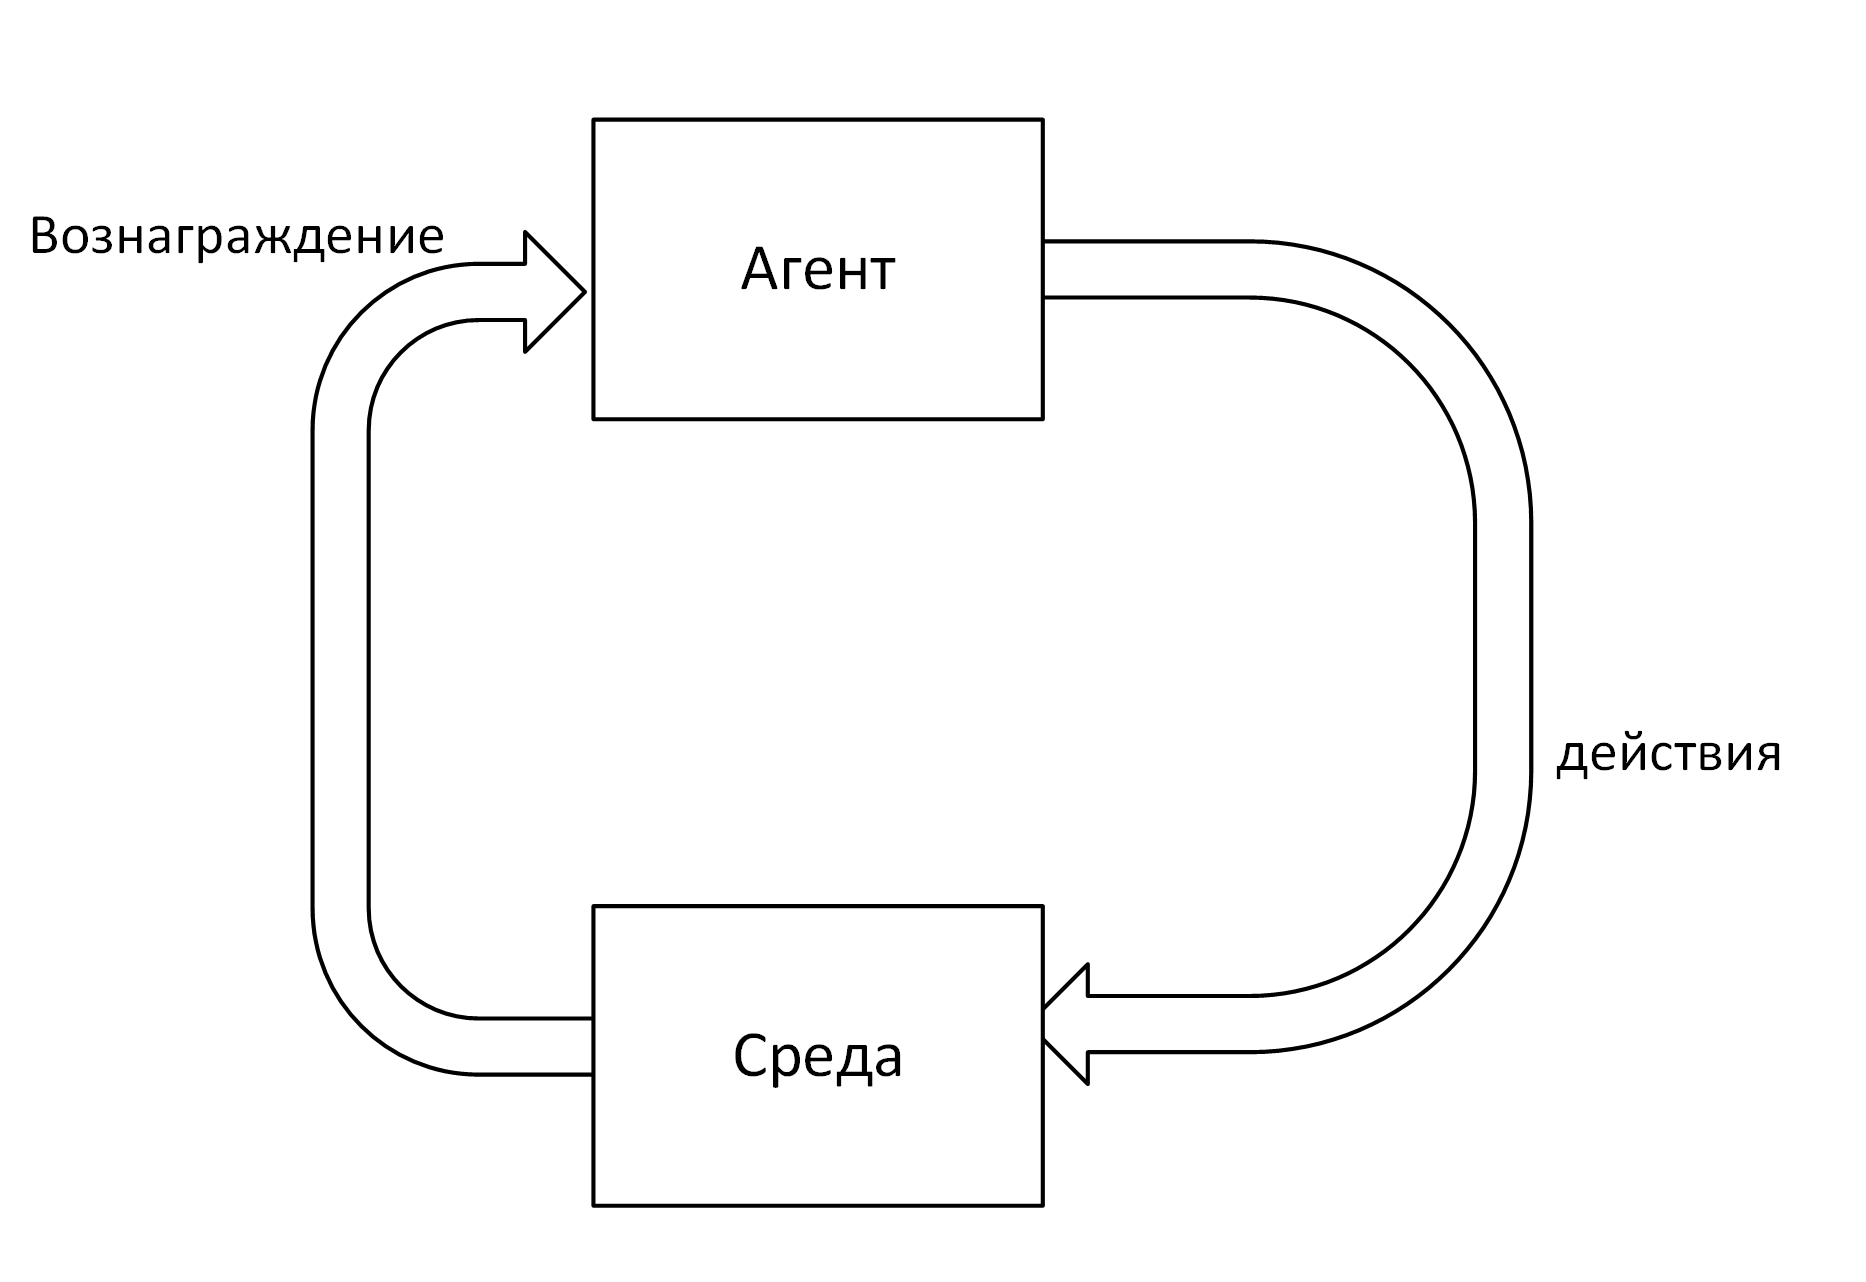
\includegraphics[scale=0.15]{figure_1}
		\caption{Общая схема взаимодействия агента со средой при обучении с подкреплением}
		\label{fig:RL_general}
	\end{figure}
	Рассмотрим пример обучения с подкреплением в среде FrozenLake. Далее эта среда будет использована для проведения практических экспериментов. В даннном случае среда дискретна, а обучение состоит из эпизодов. Мир предстваляет собой доску с 16 клетками (таблица \ref{table:Grid_world})
	\begin{table}[htb]
		\centering
		\begin{TAB}(e,1cm,1cm)[5pt]{|c|c|c|c|}{|c|c|c|c|}% (rows,min,max)[tabcolsep]{columns}{rows}
			S 	&  		&   	&   \\
				& 	H 	&  		&  H \\
				&	 	&   	&  H \\
			H 	&     	&   	&  G \\
		\end{TAB} 
		\caption{Среда FrozenLake. Символом S обозначено начальное положение агента, G -- цель, H -- полыньи}
		\label{table:Grid_world}
	\end{table}
	
	Агент начинает игру в левой верхней клетке, его задача дойти до нижней правой клетки, при этом на его пути в некоторых клетках находится полыньи, в которые он может провалиться. Если агент достигает цели, он получает вознаграждение $r$ равное 1 и эпизод заканчивается. Если агент проваливается в прорубь, то его вознаграждение $r=0$, и эпизод также заканчивается. Агент может выбирать в каком направлении ему двигаться: вверх, вниз, влево или вправо.  Таким образом, \textbf{пространство действий} агента $ A $ содержит 4 действия. Пространство наблюдений -- это индекс клетки, в которой находится агент (т.е число от 0 до 15). 
	Когда агент совершает действие из-за скользкости поверхности существует три варианта развития событий: агент попадает либо на клетку в направлении действия, либо на клетки перпендикулярные направлению выбранного действия. Например, если агент совершает действие "вверх":
	\begin{enumerate}
	\item C вероятностью 0.33 агент попадает в клетку, которая находится выше.
	\item C вероятностью 0.33 агент попадает в клетку, которая находится правее.
	\item C вероятностью 0.33 агент попадает в клетку, которая находится левее.
	\end{enumerate}
	Состояние системы -- характеристика системы в момент ее функционирования. В случае FrozenLake пространство наблюдений совпадает с пространством состояний. 
	
	В среде FrozenLake результат зависит только от текущего положения и будущих действий агента, и не зависит от состояний, которые предшествовали текущему состоянию. Другими словами, для принятия решения не важно, каким образом мы попали в текущее состояние. Процессы принятия решения, обладающие этим свойством называются \textbf{Марковскими процессами принятия решений}.
	\textbf{Стратегия} -- это некоторый набор правил (в широком смысле, поскольку агент может оперировать сложной внутренней моделью среды), которые управляют поведением агента.
	Стратегия агент может задавать недетерменированое поведение агента, т.е. она задает вероятность выполнения агентом действия $a$ в состоянии $s$:
	\begin{equation}
	\pi (a|s)=P(A_t=a|S_t=s)
	\end{equation} 
	Для марковского процесса принятия решений для каждого эпизода \textbf{отдача} на шаге \textit{t} определяется по формуле:
	\begin{equation}
		G_t = r_{t+1} + \gamma r_{t+2} + ... = \sum_{k=0}^{\inf} \gamma^k r_{t+k+1},
	\end{equation}
	где коээфициент $0 < \gamma =< 1$ вводится для того, чтобы уменьшить вклад сильно отсроченных вознаграждений. Теперь можно определить \textbf{ценность состояния}: 
	\begin{equation}
	V(s) = \mathbb{E}[G_t|S_t=s] = \mathbb{E}[\sum_{k=0}^{\inf}r_t \gamma^t].
	\end{equation}
	Таким образом, для каждого состояния s, ценность V(s) -- это средняя (ожидаемая) отдача. Ценность состояний зависит от стратегии поведения агента. 
	Для среды FrozenLake и адекватных стратегий поведения при $\gamma < 1$ клетки, которые находятся ближе к цели будут иметь большую ценность, поскольку позволяют получить вознаграждение за меньшее количество шагов.\\
	
	\subsection{Уравнение оптимальности Беллмана}
	В детерменированном случае (если выбранное действие однозначно определяет будущее состояние), чтобы выбрать наилучшее действие из состояния $S_0$ агент должен выбирать действие $a$, которое приводит к состоянию $ S_a $ с максимальной ценностью. Таким образом, ценность состояния $S_0$:
	\begin{equation}
	V(S_0) = max_{a}(r_a + \gamma V(S_a)),
	\label{eq:next_value}
	\end{equation}
	где $r_a$ -- вознаграждение за переход из состояния $ S_0 $ в состояние  $ S_a $ (для FrozenLake большая всем переходам соответсвует нулевое вознаграждение, кроме перехода в правую нижнюю клетку, для которого $r_a = 1$).
	Беллман показал, что выбор действий в соответсвии с оценкой состояния \eqref{eq:next_value} является оптимальным, т.е. позволяет получить максимальное возможное ожидаемое вознаграждение.
	В случае среды (подобно FrozenLake), которая является недетерменированной уравнение \eqref{eq:next_value} принимает вид:
	\begin{equation}
		V(S_0) = max_{a \in A}\mathbb{E}_s(r_a + \gamma V(S_a))=max_{a \in A}\sum_{s \in S}P_{a,S_0 \rightarrow s}(r_{s,a} + \gamma V_s),
	\end{equation}
	где $ P_{a,S_0 \rightarrow s} $ -- это вероятность перехода в состояние $ s $ из состояния $ S_0 $ при выполнении действия $ a $.
	Введем меру ценности действий $ Q(s,a) $, которая может быть определена через $ V(s) $:
	\begin{equation}
	Q_{s,a} = \mathbb{E}_{s'}[r_{s,a} + \gamma V_{s'}] = \sum_{s' \in S} p_{a,s \rightarrow s'}(r_{s,a} + \gamma V_{s'}).
	\end{equation}
	Также и $ V(s) $ может быть определена через $ Q(s,a) $:
	\begin{equation*}
	V_s = \max_{a \in A} Q(s,a).
	\end{equation*}
	
	Наконец, аналогичным образом с ценностью состояния, может быть рекурсивно выведено значение ценности действия:
	\begin{equation}
	Q(s,a)=r_{s,a} + \gamma \max_{a' \in A}Q(s',a')
	\end{equation}
	\subsection{Алгоритм итерации по ценностям действий}
%	\texttt{\texttt{\textbf{Алгоритм итерации по ценностям состояний} может быть описан следующей последовательностью шагов:
%	\begin{enumerate}
%		
%		\item Инциализировать ценности всех состояний $ V_i $ нулями.
%		
%		\item Для каждого состояния s обновить ценность, согласно уравнению Беллмана: 
%		\begin{equation}V_s \leftarrow \max_a \sum_{s'}p_{a,s \rightarrow s'}(r_{s,a} + \gamma V_{s'})\end{equation}
%		
%		\item Повторять шаг 2, пока изменения не станут пренебрежимо малыми.
%		
%	\end{enumerate}}}
	
	
	\textbf{Алгоритм итераций по ценностям действий} (т.е. Q) может быть описан следующей последовательностью шагов:
	
	\begin{enumerate}
		
		\item Инициализировать $ Q_{s,a} $ нулями.
		
		\item Для каждого состояния s и каждого действия a в этом состоиянии сделать обновление: 
		\begin{equation}
		Q_{s,a} \leftarrow \sum_{s'}p_{a,s \rightarrow s'}(r_{s,a} + \gamma \max_{a'}Q_{s',a'})
		\label{eq:bell_upd}
		\end{equation}
		\item Повторять шаг 2, пока изменения не станут пренебрежимо малыми.
		
	\end{enumerate}
	На практике метод имеет ограничения, связанные с пространством состояний (т.к. приходится перебирать все возможные). Кроме того, вероятности перехода из одного состояния в другое также редко когда бывают доступны напрямую. Однако имея возможность многократно "запускать" агента в среде, мы можем аппроксимировать эти значения на основании опыта (см. раздел 4).
	 
	\section{Экспериментальная часть}
	В данной работе необходимо выучить алгоритм поведения в среде с помощью алгоритма итерации по ценностям действий. Работа состоит из следующих шагов.
	\begin{enumerate}
	\item Реализовать алгоритм итерации по ценностям дейсвий и обучить агента функционированию в среде FrozenLake с помощью библиотеки gym. 
	\item Проанализровать поведение обученного агента.
	\item Повторить эксперименты с коэффициент $ \gamma  = 0.99$ и $ \gamma  = 0.7$. 
	\item Сделать выводы.
	\end{enumerate}
	Для выполнения экспериментов рекомендуется использовать Python 3.7. 
	\subsection{Библиотека для обучения с подкреплением gym}
	
	Для выполнения работы будет использоваться библиотека для обучения с подкреплением gym. Эта библиотека содержит в себе множество сред для разработки алгоритмов обучения с подкреплением. 
	Каждая среда предоставляет следующую информацию и функциональность:
	\begin{enumerate}
	\item Набор действий, которые могут быть выполнены.
	\item Метод step, чтобы выполнить действие, получить наблюдение и вознаграждение и информацию о том, закончился ли эпизод.
	\item Метод reset, который возвращает среду в исходное состояние.
	\end{enumerate}
	 
	\subsection{Сокращенный пример выполнения работы}
	Cначала импортируем все необходимые библиотеки. 
	\begin{lstlisting}[language=Python]
		import gym
		import collections
		from tensorboardX import SummaryWriter
		import os
		import shutil
	\end{lstlisting}
	Объявим главные глобальные переменные, которые будут отвечать за название среды gym, коэффициент $ \gamma $ и количество эпизодов, по которым мы будем измерять статистику.
	\begin{lstlisting}	
		ENV_NAME = "FrozenLake-v0"
		GAMMA = 0.9
		TEST_EPISODES = 20
	\end{lstlisting}
	
	Всего будем использовать три важные структуры для реализации алгоритма:
	\begin{enumerate}
	\item Таблицу вознаграждений, которая представляет собой словарь Python, с составным ключом \textit{(состояние, действие)}. Таблица содержит значения моментальных вознагражедений $ r $.
	\item Таблица переходов, которая также представляет собой словарь с составным ключом \textit{(исходное состояние, действие)}, однако в данном случае значением является еще один словарь, окторый отображает \textit{состояние назначения} в число -- количество переходов в это состояние, при выполнение действия из исходного состояния. Значения таблицы переходов позволят аппроксимировать значения вероятностей из уравнения \eqref{eq:bell_upd}
	\item Q-таблица -- таблица ценности действий, на основании которой легко описать стратегию поведения агента.
	\end{enumerate}
	
	Зададим класс агента и опишем поля, соответсвующие среде и структурам, описанным выше:
	\begin{lstlisting}	
		class Agent:
		  def __init__(self):
		    self.env = gym.make(ENV_NAME)
		      self.state = self.env.reset()
		      self.reward_table = collections.defaultdict(float)
		      self.transition_table = \
			      collections.defaultdict(collections.Counter)  
		      self.Q = collections.defaultdict(float)
	\end{lstlisting}
	
	Теперь определим функцию агента \verb|play_n_random_steps|, с помощью которой будем случайным образом выполнять действия, чтобы можно было собирать информацию о среде и заполнять структуры, описанные выше. Для этого мы используем встроенную команду из gym -- \verb|env.action_space.sample| случайным образом выбирающую одно из возможных действий.
		

	\begin{lstlisting}	
    def play_n_random_steps(self, count):
	    for _ in range(count):
		    action = self.env.action_space.sample()
		    new_state, reward, is_done, _ = self.env.step(action)
		    self.reward_table[(self.state, action, new_state)] = reward
		    self.transition_table[(self.state, action)][new_state] += 1
		    self.state = self.env.reset() if is_done else new_state
	\end{lstlisting}
	
	Также зададим функцию, которая выбирает оптимальное действие в соответсвии с текущим содержимым Q-таблицы:
	
	\begin{lstlisting}	
    def select_action(self, state):
	    best_action, best_value = None, None
	    for action in range(self.env.action_space.n):
		    action_value = self.Q[(state, action)]
		    if best_value is None or best_value < action_value:
			    best_value = action_value
			    best_action = action
    return best_action
	\end{lstlisting}
	
	Для тестирования качества обучения будем использовать следующую функцию. Она принимает на вход среду (для тестирования будем использовать отдельную), а также флаг \verb|do_rendering|, с помощью которого мы сможем осуществить пошаговый вывод состояния и действий обученного агента. 
	\begin{lstlisting}
def play_episode(self, env, do_rendering=False):
    total_reward = 0.0
    state = env.reset()
    while True:
	    action = self.select_action(state)
	    new_state, reward, is_done, _ = env.step(action)
	    if do_rendering:
		    env.render()
	    self.reward_table[(state, action, new_state)] = reward
	    self.transition_table[(state, action)][new_state] += 1
	    total_reward += reward
	    if is_done:
		    break
	    state = new_state
    return total_reward
	\end{lstlisting}
	
	Определим функцию для обновления Q-значений (ценностей действия), хранящихся в таблице:
\begin{lstlisting}
 def Q_iteration(self):
	for state in range(self.env.observation_space.n):
		for action in range(self.env.action_space.n):
			action_value = 0.0
			target_counts = self.transition_table[(state, action)]
			total = sum(target_counts.values())
			for tgt_state, count in target_counts.items():
				reward = self.reward_table[(state, action, tgt_state)]
				best_action = self.select_action(tgt_state)
					action_value += \
					(count / total) * \
				(reward + GAMMA * self.Q[(tgt_state, best_action)])
			self.Q[(state, action)] = action_value
	\end{lstlisting}
В коде выше в соответсвии с алгоритмом, мы обходим все возможные состояния и все возможные действия. Для того, чтобы применить уравнение \eqref{eq:bell_upd} мы аппроксимируем вероятности перехода из одного состояния в другое $ p_{a,s \rightarrow s'} $,  анализируя соответсвующие значения в таблице переходов. \\

Наконец, реализуем основной модуль обучения. Будем использовать tensorboard для того, чтобы отслеживать изменение вознаграждения на тесте:
\begin{lstlisting}
if __name__ == "__main__":
	test_env = gym.make(ENV_NAME)
	agent = Agent()
	writer = SummaryWriter(comment="-q-iteration")
	
	iter_no = 0
	best_reward = 0.0
	while True:
		iter_no += 1
		agent.play_n_random_steps(100)
		agent.Q_iteration()
		
		reward = 0.0
		for _ in range(TEST_EPISODES):
			reward += agent.play_episode(test_env)
			reward /= TEST_EPISODES
			writer.add_scalar("reward", reward, iter_no)
			if reward > best_reward:
				print("Best reward updated {} -> {}".format( \
					best_reward, reward))
				best_reward = reward
			if reward > 0.80:
				print("Solved in %d iterations!" % iter_no)
				break
\end{lstlisting}

В коде выше мы инициализиуем агента, а после этого в бесконечном цикле собираем статистику о среде и на основании этой статистики уточняем значения ценности действий. Каждую итерацию мы также проводим тестирование таблицы ценности действий путем измерения вознаграждения, если среднее значение больше 0.8, то мы считаем, что агент функционирует в среде корректно.

В конце обучение визуализируем один эпизод функционированния обученного агента.
\begin{lstlisting}
    env = gym.make(ENV_NAME)
    agent.play_episode(env, True)
\end{lstlisting}

При выполнении этих команд в коносли в мнемонической форме отборажается последовательность предпринятых действий и результирующих состояний:
\begin{lstlisting}
  (Left)
  SFFF
  FHFH
  FFFH
  HFFG
  
  #...
\end{lstlisting}
Таким образом, первое действие агента: <влево>, что позволяет ему с вероятностью 0.33  переместиться на клетку ниже, которая находится ближе к цели, а с вероятностью 0.66 остаться в исходной клетке.
Визуализируем кривые обучения для двух вызовов (\figurename \ref{fig:curves})
\begin{figure}[h]
	\centering
	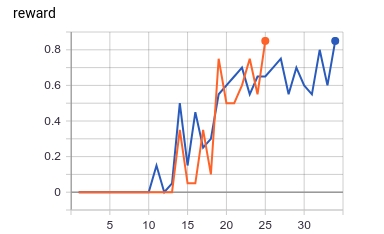
\includegraphics[scale=1]{curves}
	\caption{Кривые обучения}
	\label{fig:curves}
\end{figure}
 
	\section{Литература}
	\begin{enumerate}
	\item Lapan M. Deep Reinforcement Learning Hands-On. Birmingham: Packt Publishing. 2020. P.798 
	\item Саттон Р.С., Э.Г. Барто. Обучение с подкреплением. пер. с англ. - 2-е изд. М. : БИНОМ. Лаборатория знаний, 2014.
	\end{enumerate}
	\subsection{Вопросы для самопроверки}
	\begin{enumerate}
		\item Какие отличительные особенности обучения с подкрепления от других подходов к машинному обучения?
		\item Чем отличается ценность состояния от ценности действия?
		\item Позволяет ли алгоритм итерации по ценностям действий получать оптимальные стратегия поведения? 
		\item В чем недостатки рассмотреного алгоритма?
		\item Какова стратегия поведения агента, обученного в среде FrozenLake? Является ли она оптимальной?
		\item Можно ли обучить агента так, чтобы среднее вознаграждение было равно 1? Почему?
		
	\end{enumerate}
\end{document}  % КОНЕЦ ДОКУМЕНТА !